\chapter{CƠ SỞ LÝ THUYẾT} % Tên của chương

\label{Chapter2} % Để trích dẫn chương này ở chỗ nào đó trong bài, hãy sử dụng lệnh \ref{Chapter1} 

%----------------------------------------------------------------------------------------

% Định nghĩa một số lệnh cần thiết để điều chỉnh định dạng cho một số nội dung nhất định trong bài
\renewcommand{\keyword}[1]{\textbf{#1}}
\renewcommand{\tabhead}[1]{\textbf{#1}}
\renewcommand{\code}[1]{\texttt{#1}}
\renewcommand{\file}[1]{\texttt{\bfseries#1}}
\renewcommand{\option}[1]{\texttt{\itshape#1}}
\setcounter{secnumdepth}{3} 

\section{Mô hình phát hiện đối tượng YOLO}

YOLO là 1 từ viết tắt cho ‘You only look once’ (Bạn chỉ nhìn một lần) là một thuật toán phát hiện đối tượng chia hình ảnh thành một hệ thống lưới. Mỗi ô trong lưới chịu trách nhiệm phát hiện các đối tượng trong chính nó. YOLO là một trong những thuật toán phát hiện đối tượng nổi tiếng nhất do tốc độ và độ chính xác của nó. 

YOLO là một mô hình mạng CNN cho việc phát hiện, nhận dạng, phân loại đối tượng. YOLO được tạo ra từ việc kết hợp giữa các convolutional layers và connected layers. Trong đó các convolutional layers sẽ trích xuất ra các feature của ảnh, còn fullconnected layers sẽ dự đoán ra xác suất đó và tọa độ của đối tượng.

\begin{figure}[H]
    \centering
    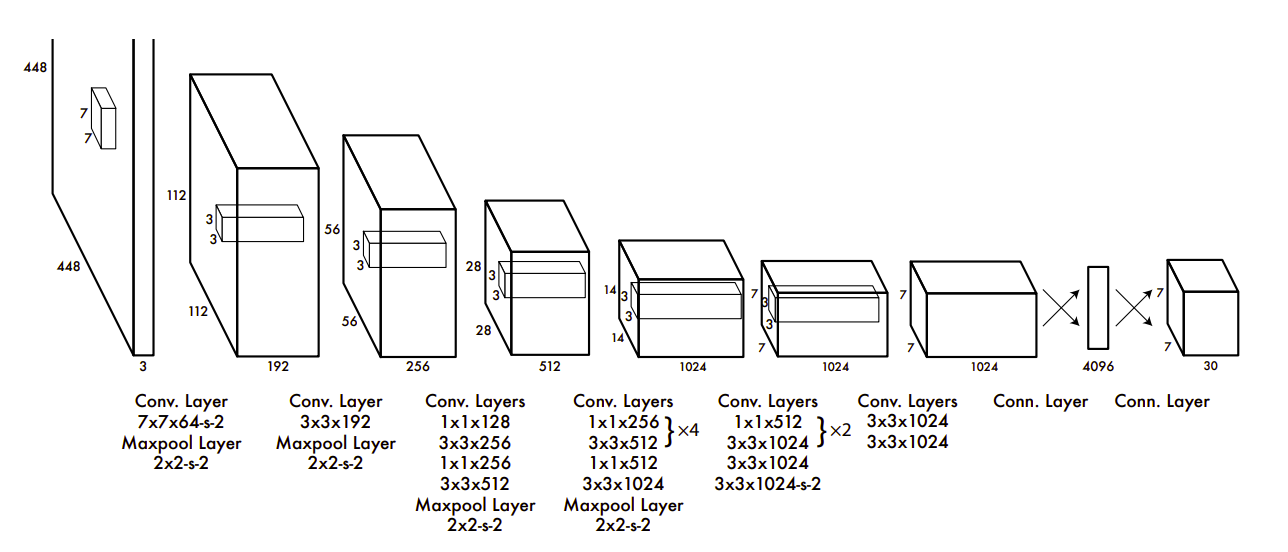
\includegraphics[width=0.9\linewidth]{Figures/Chapter 2/Chapter3_2.png}
    \caption{Mô hình mạng CNN được sử dụng trong YOLO}
    \label{yolo:chapter2}
\end{figure}

Hình ảnh đầu vào sẽ được chia thành một lưới kích thước $S \times S$, trong đó mỗi ô lưới chịu trách nhiệm phát hiện các đối tượng có tâm nằm trong ô đó. Đối với mỗi ô, mô hình sẽ dự đoán một số lượng bounding box cùng với thông tin về vị trí và xác suất lớp.

Với mỗi bounding box, mô hình dự đoán 5 tham số bao gồm $(x, y, w, h, confidence)$. Trong đó, $(x, y)$ là tọa độ tâm của bounding box tương đối so với ô lưới, còn $(w, h)$ là chiều rộng và chiều cao được chuẩn hóa theo kích thước toàn ảnh. Giá trị $confidence$ thể hiện mức độ tin cậy của bounding box, được tính dựa trên xác suất tồn tại đối tượng và độ chồng lắp giữa bounding box dự đoán và ground truth.

Ngoài ra, mỗi ô lưới còn dự đoán xác suất thuộc về các lớp đối tượng dưới dạng $Pr(Class_i \mid Object)$. Xác suất cuối cùng của một lớp được tính bằng cách kết hợp giữa xác suất lớp và $confidence$ của bounding box.

\subsection{Mô hình YOLO26}

YOLO26 (hay YOLOv26) là thế hệ mới nhất thuộc họ mô hình phát hiện đối tượng You Only Look Once (YOLO) do Ultralytics phát triển, được giới thiệu vào khoảng cuối năm 2025. Khác với các phiên bản trước chủ yếu tập trung vào việc gia tăng độ chính xác thông qua việc mở rộng kích thước mô hình, YOLO26 được thiết kế lại nhằm tối ưu hóa cho việc triển khai trên các thiết bị biên (edge devices), hệ thống nhúng và môi trường có tài nguyên hạn chế.

\begin{figure}[H]
    \centering
    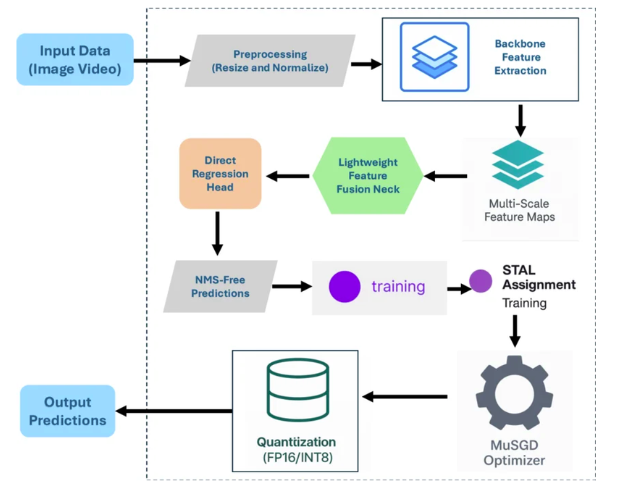
\includegraphics[height=8cm, keepaspectratio]{Figures/Chapter 2/Chapter2_9.png}
    \caption{Kiến trúc tổng quan YOLO26}
    \label{yolo26:chapter2}
\end{figure}


\subsubsection*{1. Kiến trúc NMS-Free}

Các phiên bản YOLO trước đây (như YOLOv8, YOLOv9) yêu cầu bước hậu xử lý Non-Maximum Suppression (NMS) để loại bỏ các bounding box trùng lặp. Tuy nhiên, YOLO26 được thiết kế theo hướng end-to-end hoàn chỉnh, cho phép mô hình trực tiếp xuất ra các dự đoán cuối cùng mà không cần áp dụng NMS.

Việc loại bỏ bước NMS giúp giảm độ trễ của toàn hệ thống và đơn giản hóa pipeline suy luận, đặc biệt phù hợp với các ứng dụng thời gian thực.

\begin{figure}[H]
    \centering
    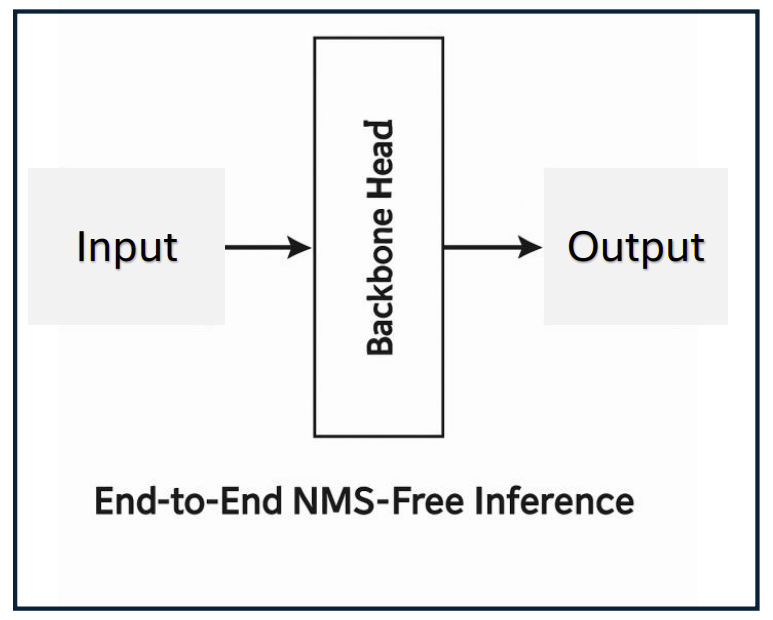
\includegraphics[height=5cm, keepaspectratio]{Figures/Chapter 2/Chapter2_4.png}
    \caption{Kiến trúc NMS-Free}
    \label{NMS:chapter2}
\end{figure}

\subsubsection*{2. Loại bỏ Distribution Focal Loss}

Trong các phiên bản trước, Distribution Focal Loss (DFL) được sử dụng để cải thiện độ chính xác của bounding box. Tuy nhiên, DFL gây khó khăn trong việc chuyển đổi mô hình sang các định dạng triển khai như TensorRT, ONNX hay CoreML.

YOLO26 loại bỏ hoàn toàn DFL, giúp quá trình export và triển khai mô hình trở nên đơn giản, ổn định và tương thích tốt hơn với phần cứng.

\begin{figure}[H]
    \centering
    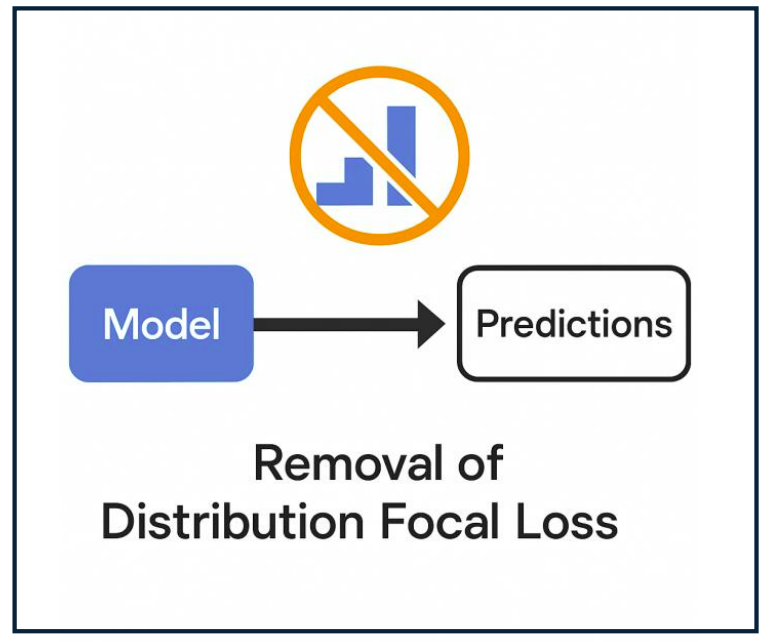
\includegraphics[height=5cm, keepaspectratio]{Figures/Chapter 2/Chapter2_5.png}
    \caption{Loại bỏ DFL}
    \label{DFL:chapter2}
\end{figure}

\subsubsection*{3. Tối ưu phát hiện vật thể nhỏ}

YOLO26 áp dụng cơ chế gán nhãn mới mang tên Small-Target-Aware Label Assignment (STAL), kết hợp với hàm mất mát cải tiến. Cơ chế này giúp mô hình nhạy hơn với các vật thể nhỏ hoặc ở khoảng cách xa.

Nhờ đó, hiệu năng phát hiện các đối tượng nhỏ như biển số xe hoặc chi tiết chữ viết tay được cải thiện đáng kể so với các phiên bản trước.

\begin{figure}[H]
    \centering
    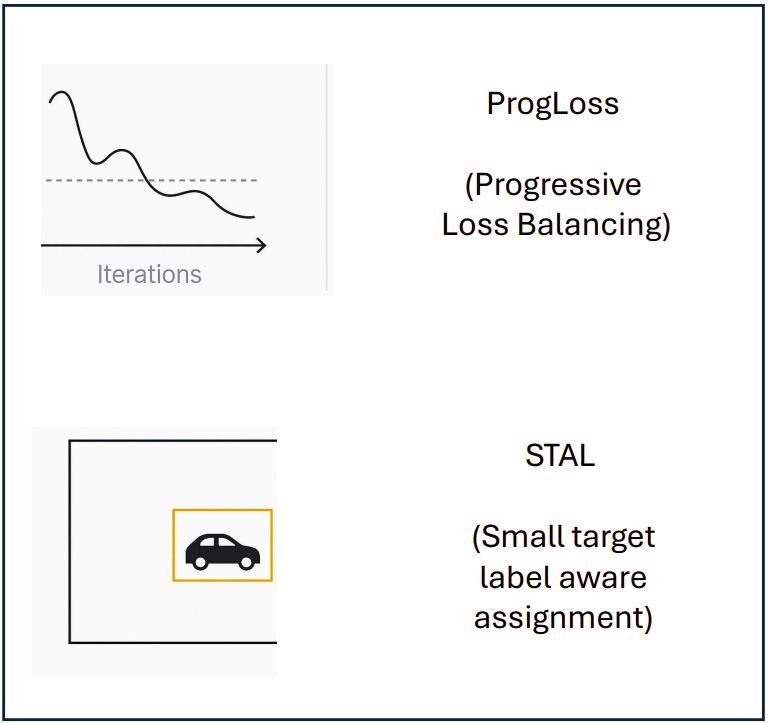
\includegraphics[height=5cm, keepaspectratio]{Figures/Chapter 2/Chapter2_6.png}
    \caption{Tối ưu cho vật thể nhỏ}
    \label{STAL:chapter2}
\end{figure}


\subsubsection*{4. Trình tối ưu hóa MuSGD}

YOLO26 sử dụng trình tối ưu hóa MuSGD, kết hợp giữa Stochastic Gradient Descent (SGD) và thuật toán Muon. Phương pháp này giúp cải thiện tốc độ hội tụ và đảm bảo sự ổn định trong quá trình huấn luyện.

Việc áp dụng MuSGD cho phép mô hình đạt hiệu năng cao mà vẫn duy trì độ ổn định khi huấn luyện trên các tập dữ liệu lớn.

\begin{figure}[H]
    \centering
    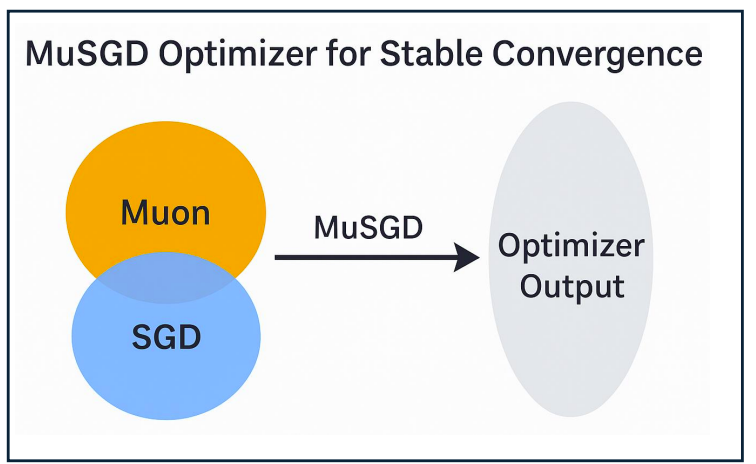
\includegraphics[height=5cm, keepaspectratio]{Figures/Chapter 2/Chapter2_7.png}
    \caption{Tối ưu hóa MuSGD}
    \label{MuSGD:chapter2}
\end{figure}

Nhờ đó, YOLO26 có thể được sử dụng như một nền tảng thống nhất cho nhiều ứng dụng khác nhau trong thị giác máy tính.

\section{Ước lượng chiều sâu từ ảnh đơn với mô hình MiDaS}

\subsection{Bài toán Monocular Depth Estimation}

Ước lượng chiều sâu từ ảnh đơn (Monocular Depth Estimation) là quá trình dự đoán khoảng cách của các vật thể trong một bức ảnh 2D so với góc nhìn của camera, mà không cần sử dụng đến hệ thống camera kép (Stereo camera) hay các cảm biến không gian chuyên dụng như LiDAR. Đối với hệ thống hỗ trợ người khiếm thị SmartNav, việc áp dụng bài toán này mang ý nghĩa cốt lõi, cho phép hệ thống phân tích và ước lượng khoảng cách của chướng ngại vật ngay trên các thiết bị di động có cấu hình phần cứng giới hạn.

Thay vì trả về giá trị khoảng cách tuyệt đối tính bằng mét, đầu ra của mô hình thường là một bản đồ thị sai (Disparity Map). Trong bản đồ này, giá trị điểm ảnh (pixel) càng lớn biểu thị vật thể càng gần camera, và ngược lại. Khó khăn lớn nhất của bài toán này nằm ở tính nhập nhằng (ambiguity) của không gian 2D, khi một vật thể nhỏ ở gần có thể tạo ra hình chiếu trên cảm biến tương đương với một vật thể lớn ở xa.

\subsection{Kiến trúc mô hình MiDaS}

Để giải quyết thách thức trên, hệ thống SmartNav ứng dụng mô hình MiDaS (Multiple Depth Estimation Datasets), một mạng nơ-ron được huấn luyện trên nhiều bộ dữ liệu khác nhau để đảm bảo khả năng tổng quát hóa tốt nhất trên mọi môi trường thực tế như trong nhà, ngoài trời và đường phố đô thị.

% ==========================================
% CHỖ NÀY CHÈN ẢNH MIDAS (RGB VÀ DEPTH MAP)
% ==========================================
\begin{figure}[H]
    \centering
    % Đổi tên file 'midas_depth.png' thành tên file ảnh thực tế của ông
    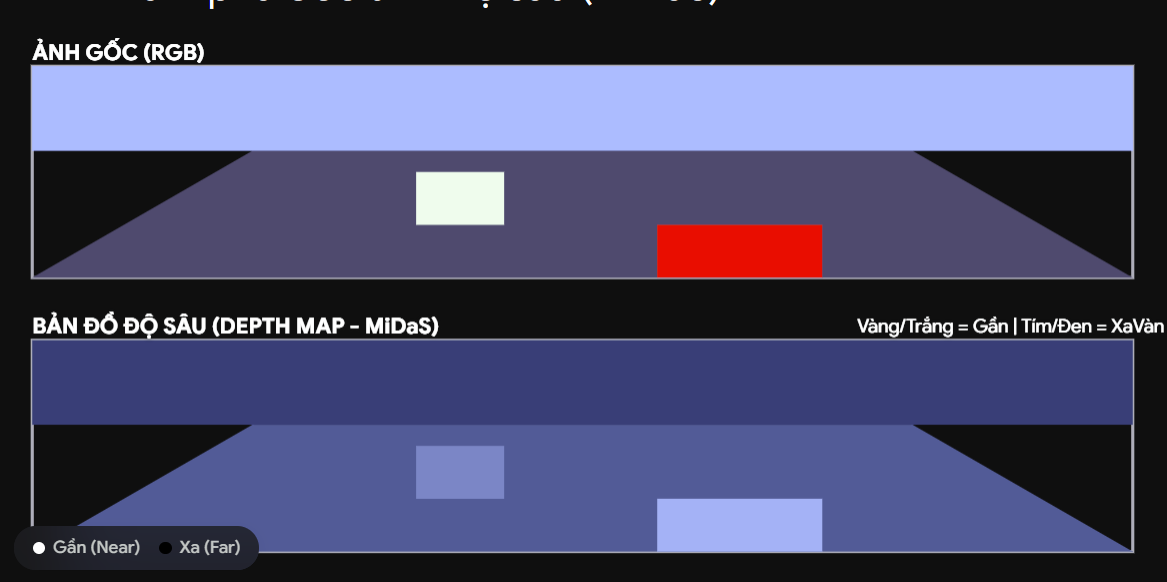
\includegraphics[width=0.9\linewidth]{Figures/Chapter 2/midas_depth.png}
    \caption{So sánh ảnh RGB gốc và bản đồ độ sâu (Depth Map) được trích xuất từ mô hình MiDaS}
    \label{fig:midas_architecture}
\end{figure}

Trong dự án này, phiên bản MiDaS loại nhỏ (\texttt{MiDaS\_small}) được lựa chọn nhằm tối ưu hóa tốc độ xử lý trên CPU và các thiết bị biên (Edge Devices). Quá trình xử lý độ sâu được thực hiện thông qua các bước chính:

\begin{itemize}
    \item \textbf{Tiền xử lý và Nội suy:} Hình ảnh RGB đầu vào được chuẩn hóa bằng hàm biến đổi đặc thù của MiDaS, sau đó được đưa qua mạng nơ-ron để dự đoán bản đồ thị sai. Kết quả đầu ra được nội suy bậc ba (Bicubic Interpolation) để đồng bộ lại với kích thước khung hình gốc của camera.
    
    \item \textbf{Chuẩn hóa Min-Max (Min-Max Normalization):} Nhằm tạo ra một thang đo đồng nhất cho thuật toán cảnh báo, bản đồ thị sai được chuẩn hóa về dải giá trị từ 0 đến 1. Trong đó, mức $1.0$ đại diện cho điểm gần nhất và $0.0$ là điểm xa nhất ở đường chân trời.
    
    \item \textbf{Lọc nhiễu bằng Bách phân vị (Percentile Filtering):} Khi hệ thống nhận diện được một vật cản (thông qua Bounding Box từ mô hình YOLO26), một vùng không gian tương ứng trên bản đồ độ sâu sẽ được trích xuất. Để loại bỏ nhiễu từ phông nền (background noise), hệ thống không sử dụng giá trị trung bình mà tính toán Bách phân vị thứ 80 (80th Percentile) của vùng không gian đó. Phương pháp này đảm bảo chỉ những điểm ảnh thuộc bề mặt lồi lên của chướng ngại vật mới được lấy làm điểm số khoảng cách cuối cùng, giúp tăng độ tin cậy của cảnh báo.
\end{itemize}


\section{Theo dõi đa vật thể (Multi-Object Tracking) với thuật toán Centroid Tracking}

\subsection{Vai trò của bài toán theo dõi vật thể}

Nhận diện vật thể (Object Detection) chỉ cung cấp thông tin không gian rời rạc tại từng khung hình riêng lẻ. Để đánh giá được mức độ nguy hiểm của một phương tiện đang di chuyển, hệ thống cần có khả năng "ghi nhớ" và liên kết các kết quả nhận diện của cùng một phương tiện đó xuyên suốt nhiều khung hình liên tiếp. Quá trình gán và duy trì định danh (ID) cố định này được gọi là Theo dõi Đa vật thể (Multi-Object Tracking - MOT).

\subsection{Thuật toán Centroid Tracking}

Trong hệ thống SmartNav, module theo dõi vật thể đóng vai trò then chốt trong việc phân tích véc-tơ chuyển động (Motion Vector) để xác định vật cản đang tiến lại gần hay ra xa người dùng. Hệ thống áp dụng thuật toán theo dõi tâm (Centroid Tracking) tối ưu cho tốc độ cao. 

% ==========================================
% CHỖ NÀY CHÈN ẢNH MINH HỌA TRACKING
% ==========================================
\begin{figure}[H]
    \centering
    % Đổi tên file 'centroid_tracking.png' thành tên file ảnh thực tế của ông
    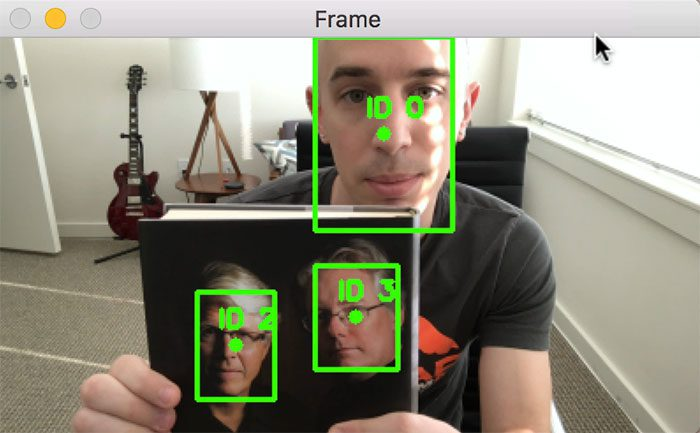
\includegraphics[width=0.8\linewidth]{Figures/Chapter 2/centroid_tracking.png}
    \caption{Minh họa thuật toán Centroid Tracking tính toán khoảng cách Euclid giữa hai khung hình liên tiếp}
    \label{fig:centroid_tracking}
\end{figure}

Quy trình hoạt động được diễn ra theo các nguyên tắc hình học cơ bản:

\begin{enumerate}
    \item \textbf{Tính toán tâm hình học (Centroid):} Từ tọa độ khung bao do YOLO26 cung cấp, hệ thống xác định điểm tâm của vật thể trên không gian 2D.
    
    \item \textbf{Đo lường khoảng cách Euclid:} Khi nhận được dữ liệu khung hình mới, hệ thống tính toán khoảng cách Euclid giữa tâm của vật thể ở khung hình hiện tại và tâm của các vật thể đã được định danh ở khung hình trước đó. Khoảng cách Euclid ($d$) giữa điểm $A(x_1, y_1)$ ở khung hình trước và điểm $B(x_2, y_2)$ ở khung hình hiện tại được tính bằng công thức:
    \begin{equation}
        d = \sqrt{(x_2 - x_1)^2 + (y_2 - y_1)^2}
    \end{equation}
    
    \item \textbf{Gán định danh (ID Assignment):} Dựa trên thuật toán láng giềng gần nhất (Nearest Neighbour), nếu khoảng cách Euclid nhỏ hơn một ngưỡng cho phép (tương đương với việc vật thể chỉ di chuyển một đoạn ngắn giữa hai khung hình liên tiếp), hệ thống sẽ gán ID cũ cho vật thể mới. Ngược lại, nếu khoảng cách vượt ngưỡng, một vật thể hoàn toàn mới sẽ được cấp ID mới.
    
    \item \textbf{Duy trì vòng đời (Object Lifecycle):} Để xử lý tình huống vật cản bị che khuất tạm thời (Occlusion) rồi xuất hiện lại, hệ thống sử dụng một bộ đếm số khung hình vắng mặt. Một ID chỉ bị xóa khỏi bộ nhớ theo dõi nếu nó không xuất hiện lại sau một khoảng thời gian nhất định (ví dụ: \texttt{max\_disappeared = 30} khung hình).
\end{enumerate}

Sự kết hợp đồng bộ giữa mô hình nhận diện YOLO26, mô hình độ sâu MiDaS và thuật toán theo dõi tạo ra một tập dữ liệu không gian - thời gian hoàn chỉnh, làm tiền đề vững chắc cho việc thiết kế Khối Đánh giá Nguy hiểm (Danger Analyzer) ở chương tiếp theo.